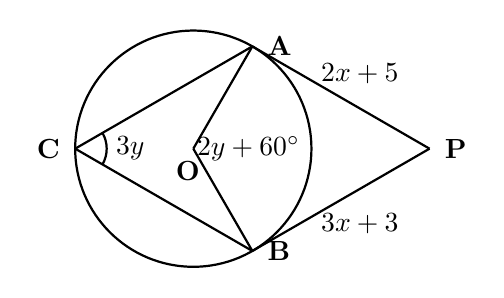
\begin{tikzpicture}[scale=1]

    % Define the center of the circle
    \coordinate (O) at (0,0);

    % Draw the circle
    \draw[thick] (O) circle (1.5);

    % Define points on the circle
    \coordinate (A) at (60:1.5);
    \coordinate (B) at (300:1.5);
    \coordinate (C) at (180:1.5);

    % Define the external point P
    \coordinate (P) at (3,0);

    % Draw the lines and segments
    \draw[thick] (C) -- (A);
    \draw[thick] (C) -- (B);
    \draw[thick] (O) -- (A);
    \draw[thick] (O) -- (B);
    \draw[thick] (P) -- (A);
    \draw[thick] (P) -- (B);

    % Draw the angle arcs
    % Arc at C (fixed to be inside)
    % The lines from C to A and B are at +30 and -30 degrees relative to C.
    \draw[thick] (C) ++(-30:0.4) arc (-30:30:0.4);

    % Add labels for the points
    \node[right, xshift=2pt] at (A) {\textbf{A}};
    \node[right, xshift=2pt] at (B) {\textbf{B}};
    \node[left, xshift=-2pt] at (C) {\textbf{C}};
    % Label O shifted a tiny bit down-right from the center
    \node[xshift=-2pt, yshift=-8pt] at (O) {\textbf{O}};
    \node[right, xshift=2pt] at (P) {\textbf{P}};

    % Add angle values
    \node at (180:0.8) {$3y$};
    % Shifted the 2y+60 label a tiny bit left by reducing the distance from 0.9 to 0.7
    \node at (0:0.7) {$2y+60^{\circ}$};

    % Add side length values
    \node[above right] at (1.5, 0.7) {$2x+5$};
    \node[below right] at (1.5, -0.7) {$3x+3$};

\end{tikzpicture}